\chapter{Security and User Privacy Vulnerabilities of Instant Messaging System}
\label{ch:security-and-user-privacy-vulnerabilities-of-instant-messaging-system}

%Nowadays, the instant messaging systems became the most widely-used and convenient way of communication between
%people via internet.
%These systems offer a simple and inexpensive way to continuance existing relationships and forming new by providing an
%attractive means for sharing information and digital social interactions.
%The quick development of instant messaging systems and the widening of their popularity sometimes moves the
%focus from possible security risks.
%In the worst case, instant messaging system exposes vulnerable to security and privacy channels to hackers and intruders
%[\cite{mcclure2009hacking, mannan2005secure}].
%In existing instant messaging systems, there are multiple privacy and security issues that need to be resolved in order
%to protect user's confidential information and shared data via these messaging applications [\cite{loesing2006privacy}].
%The source [\cite{job2015modified}] gives an analysis of Telegram Messenger and the related MTProto Protocol with cryptography
%behind the popular messenger Telegram.
%Meanwhile, the researchers in [\cite{khan2015survey}] discussed types of threats on privacy of instant messaging systems
%and ranges of thereat effects for both, user and provider.
%There are numerous risks associated with the use of instant messaging applications and as with any form of
%electronic communication one must take certain steps to mitigate those risks.
%In this section we analyze security and user privacy vulnerabilities of instant messaging from the prospective of three
%actors: server, communication channel, end-user.


%\section{Server related vulnerabilities}\label{sec:server-vulnerabilities}
%\subsection{Revealing confidential information}\label{subsec:revealing-confidential-information}
Revealing confidential information over an unsecured delivery channel.
Public Instant Messaging transmits unencrypted information, so it should never be used for sensitive or confidential
information.
The information is on the Internet and may be accessed by anyone.

\subsection{Spreading viruses and worms}\label{subsec:spreading-viruses-and-worms}
Instant Message programs are fast becoming a preferred method for launching network viruses and worms.
The lack of built-in security, the ability to download files and built-in "buddy list" of recipients create an
environment in which viruses and worms can spread quickly.
The threat is growing so fast that Instant Messenger is quickly catching up to e-mail as a primary point of attack.

\subsection{Copyright infringement}\label{subsec:copyright-infringement}
Copyright infringement [\cite{hardy2002criminal}] is the use of works protected by copyright law without
permission for a usage where such permission is required, thereby infringing certain exclusive rights granted to the
copyright holder, such as the right to reproduce, distribute, display or perform the protected work, or to make
derivative works.
The copyright holder is typically the work's creator, or a publisher or other business to whom copyright has been assigned.
Copyright holders routinely invoke legal and technological measures to prevent and penalize copyright infringement.
Copyright infringement disputes are usually resolved through direct negotiation, a notice and take down process, or
litigation in civil court.
Egregious or large-scale commercial infringement, especially when it involves counterfeiting, is sometimes prosecuted
via the criminal justice system.
Shifting public expectations, advances in digital technology and the increasing reach of the Internet have led to such
widespread, anonymous infringement that copyright-dependent industries now focus less on pursuing individuals who seek
and share copyright-protected content online, and more on expanding copyright law to recognize and
penalize, as indirect infringers, the service providers and software distributors who are said to facilitate and
encourage individual acts of infringement by others.
Estimates of the actual economic impact of copyright infringement vary widely and depend on other factors.
Nevertheless, copyright holders, industry representatives, and legislators have long characterized copyright
infringement as piracy or theft -- language which some US courts now regard as pejorative or otherwise contentious,
see~\cite{powell1984dowling, li2009intellectual}.
%
%
%\section{Communication channel related vulnerabilities}\label{sec:communication-channel-vulnerabilities}
%\subsection{Exposing the network to backdoor Trojans}\label{subsec:exposing-the-network-to-backdoor-trojans}
Malware such as adware, spyware, worms, Trojans, and other viruses can easily be transmitted through the
Instant Messaging program.
This also includes phishing programs that disguise themselves as legitimate and then trick you into revealing
your personal information.

\subsection{Denial of Service Attacks}\label{subsec:denial-of-service-attacks}
In computing, a denial-of-service attack (DoS attack) is a cyber-attack in which the perpetrator seeks to make a machine or
network resource unavailable to its intended users by temporarily or indefinitely disrupting services of a host connected
to the Internet.
Denial of service is typically accomplished by flooding the targeted machine or resource with superfluous requests in
an attempt to overload systems and prevent some or all legitimate requests from being fulfilled, see~\cite{gu2007denial}.
In a distributed denial-of-service attack (DDoS attack), the incoming traffic flooding the victim originates from
many different sources.
This effectively makes it impossible to stop the attack simply by blocking a single source.
A DoS or DDoS attack is analogous to a group of people crowding the entry door of a shop, making it hard for legitimate
customers to enter, thus disrupting trade.

Criminal perpetrators of DoS attacks often target sites or services hosted on high-profile web servers such as banks or
credit card payment gateways.
Researches at~\cite{prince2016empty, halpin2012philosophy} conclude that revenge, blackmail and activism can
motivate these attacks.

\subsection{Hijacking Sessions}\label{subsec:hijacking-sessions}
In computer science, session hijacking, sometimes also known as cookie hijacking is the exploitation of a valid computer
session -- sometimes also called a session key to gain unauthorized access to information or services in a computer system.
In particular, it is used to refer to the theft of a magic cookie used to authenticate a user to a remote server.
It has particular relevance to web developers, as the HTTP cookies used to maintain a session on many web sites
can be easily stolen by an attacker using an intermediary computer or with access to the saved cookies on the victim's
computer.
After successfully stealing appropriate session cookies an adversary might use the Pass the Cookie technique to perform
session hijacking.
By~\cite{bugliesi2015cookiext}, the cookie hijacking is commonly used against client authentication on the internet.
Modern web browsers use cookie protection mechanisms to protect the web from being attacked.
A popular method is using source-routed IP packets.
This allows an attacker at point B on the network to participate in a conversation between A and C by encouraging the
IP packets to pass through B's machine.
If source-routing is turned off, the attacker can use "blind" hijacking, whereby it guesses the responses of the two
machines.
Thus, the attacker can send a command, but can never see the response.
However, a common command would be to set a password allowing access from elsewhere on the net.

An attacker can also be "inline" between A and C using a sniffing program to watch the conversation.
This is known as a "man-in-the-middle attack" [\cite{callegati2009man}].

\subsection{Cross-site request forgery}\label{subsec:cross-site-request-forgery}
Cross-site request forgery, also known as one-click attack or session riding and abbreviated as CSRF or XSRF,
is a type of malicious exploit of a website where unauthorized commands are submitted from a user that the web
application trusts [\cite{barth2008robust}].
There are many ways in which a malicious website can transmit such commands;
specially-crafted image tags, hidden forms, and JavaScript XMLHttpRequests, for example, can all work without
the user's interaction or even knowledge.
Unlike cross-site scripting (XSS), which exploits the trust a user has for a particular site,
CSRF exploits the trust that a site has in a user's browser.

In a CSRF attack, an innocent end user is tricked by an attacker into submitting a web request that they did not intend.
This may cause actions to be performed on the website that can include inadvertent client or server data leakage,
change of session state, or manipulation of an end user's account.

CSRF is also used as an abbreviation in defences against CSRF attacks, such as techniques that use header data,
form data, or cookies, to test for and prevent such attacks.

\subsection{Cross-site scripting}\label{subsec:cross-site-scripting}
Cross-site scripting (XSS) is a type of security vulnerability typically found in web applications [\cite{vogt2007cross}].
XSS attacks enable attackers to inject client-side scripts into web pages viewed by other users.
A cross-site scripting vulnerability may be used by attackers to bypass access controls such as the same-origin policy.
Cross-site scripting attacks use known vulnerabilities in web-based applications, their servers, or the plug-in systems
on which they rely.
Exploiting one of these, attackers fold malicious content into the content being delivered from the compromised site.
When the resulting combined content arrives at the client-side web browser, it has all been delivered from the trusted source,
and thus operates under the permissions granted to that system.
By finding ways of injecting malicious scripts into web pages, an attacker can gain elevated access-privileges
to sensitive page content, to session cookies, and to a variety of other information maintained by the browser on
behalf of the user.
Cross-site scripting attacks are a case of code injection.


%\section{Traits of a secure instant messenger}\label{sec:traits-of-a-secure-instant-messenger}
%In November 2014, the Electronic Frontier Foundation [\cite{von2010electronic}] listed seven traits that contribute to
the security of instant messengers:
\begin{itemize}
    \item Having communications encrypted in transit between all the links in the communication path.
    \item Having communications encrypted with keys the provider does not have access to (end-to-end encryption).
    \item Making it possible for users to independently verify their correspondent's identity by comparing key fingerprints.
    \item Having past communications secure if the encryption keys are stolen (forward secrecy).
    \item Having the source code open to independent review (open source).
    \item Having the software's security designs well-documented.
    \item Having a recent independent security audit.
\end{itemize}
In addition, the security of instant messengers may further be improved if they:
\begin{itemize}
    \item Do not log or store any information regarding any message or its contents.
    \item Do not log or store any information regarding any session or event.
    \item Do not rely on a central authority for the relaying of messages (decentralized computing).
\end{itemize}
%
%
%\section{User responsibilities}\label{sec:user-responsibilities}
%User responsibilities and procedures are as follows:
\begin{itemize}
    \item Ensure that your Instant Messaging System account password meets Carnegie Mellon
    University [\cite{shay2010encountering}] recommendations for strong passwords.
    Refer to the Guidelines for Password Management and to the Managing Your Password web pages.
    \item Download and install security upgrades from Instant Messaging System companies.
    This software is frequently updated to address security flaws.
    \item Turn on automatic updates for your Instant Messaging program and install updates as soon as they are available.
    \item Investigate encryption for your Instant Messaging client.
    The Electronic Frontier Foundation provides Instant Messaging encryption resources.
    \item Don't allow your Instant Messaging program to "remember" your password or automatically sign in to your account.
    \item Don't automatically accept incoming messages from sign-in names that are not on your contact list.
    If someone wants to begin to communicate with you via Instant Messaging System,
    they should email you or phone you to exchange Instant Messaging sign-in names.
    \item Don't accept file transfers under any circumstances.
    File transfers are an easy way for hackers to launch virus attacks and are not scanned for viruses before reaching your computer.
    In this case, sending an attachment via e-mail would be a better alternative because you
    \begin{enumerate}
        \item Expect the communication
        \item The attachment will be scanned at the mail server in addition to the anti-virus application on your computer
    \end{enumerate}
    \item Don't click links sent to you in a message, even if they appear to be from someone you know.
    Many links often go to a site hosting malware or may be malformed in such a way as to exploit another vulnerability.
    \item Protect Privacy of Sensitive Data.
    DON'T discuss via Instant Messaging System or install an Instant Messaging application on a computer containing sensitive data.
    Don't assume that your Instant Messaging conversations are private or secure.
    Most Instant Messaging programs are not encrypted.
    Therefore, someone listening on the network can read anything said in your Instant Messaging conversation.
    \item Avoid file-sharing.
    File-sharing increases the risk that unauthorized parties could gain access to the computer.
    \item Implement Virus Protection that includes network desktop and laptop solutions to handle both Instant Messaging System
    methods of delivery (Server Broker and Server Proxy).
\end{itemize}

\begin{figure}[H]
    \centering
    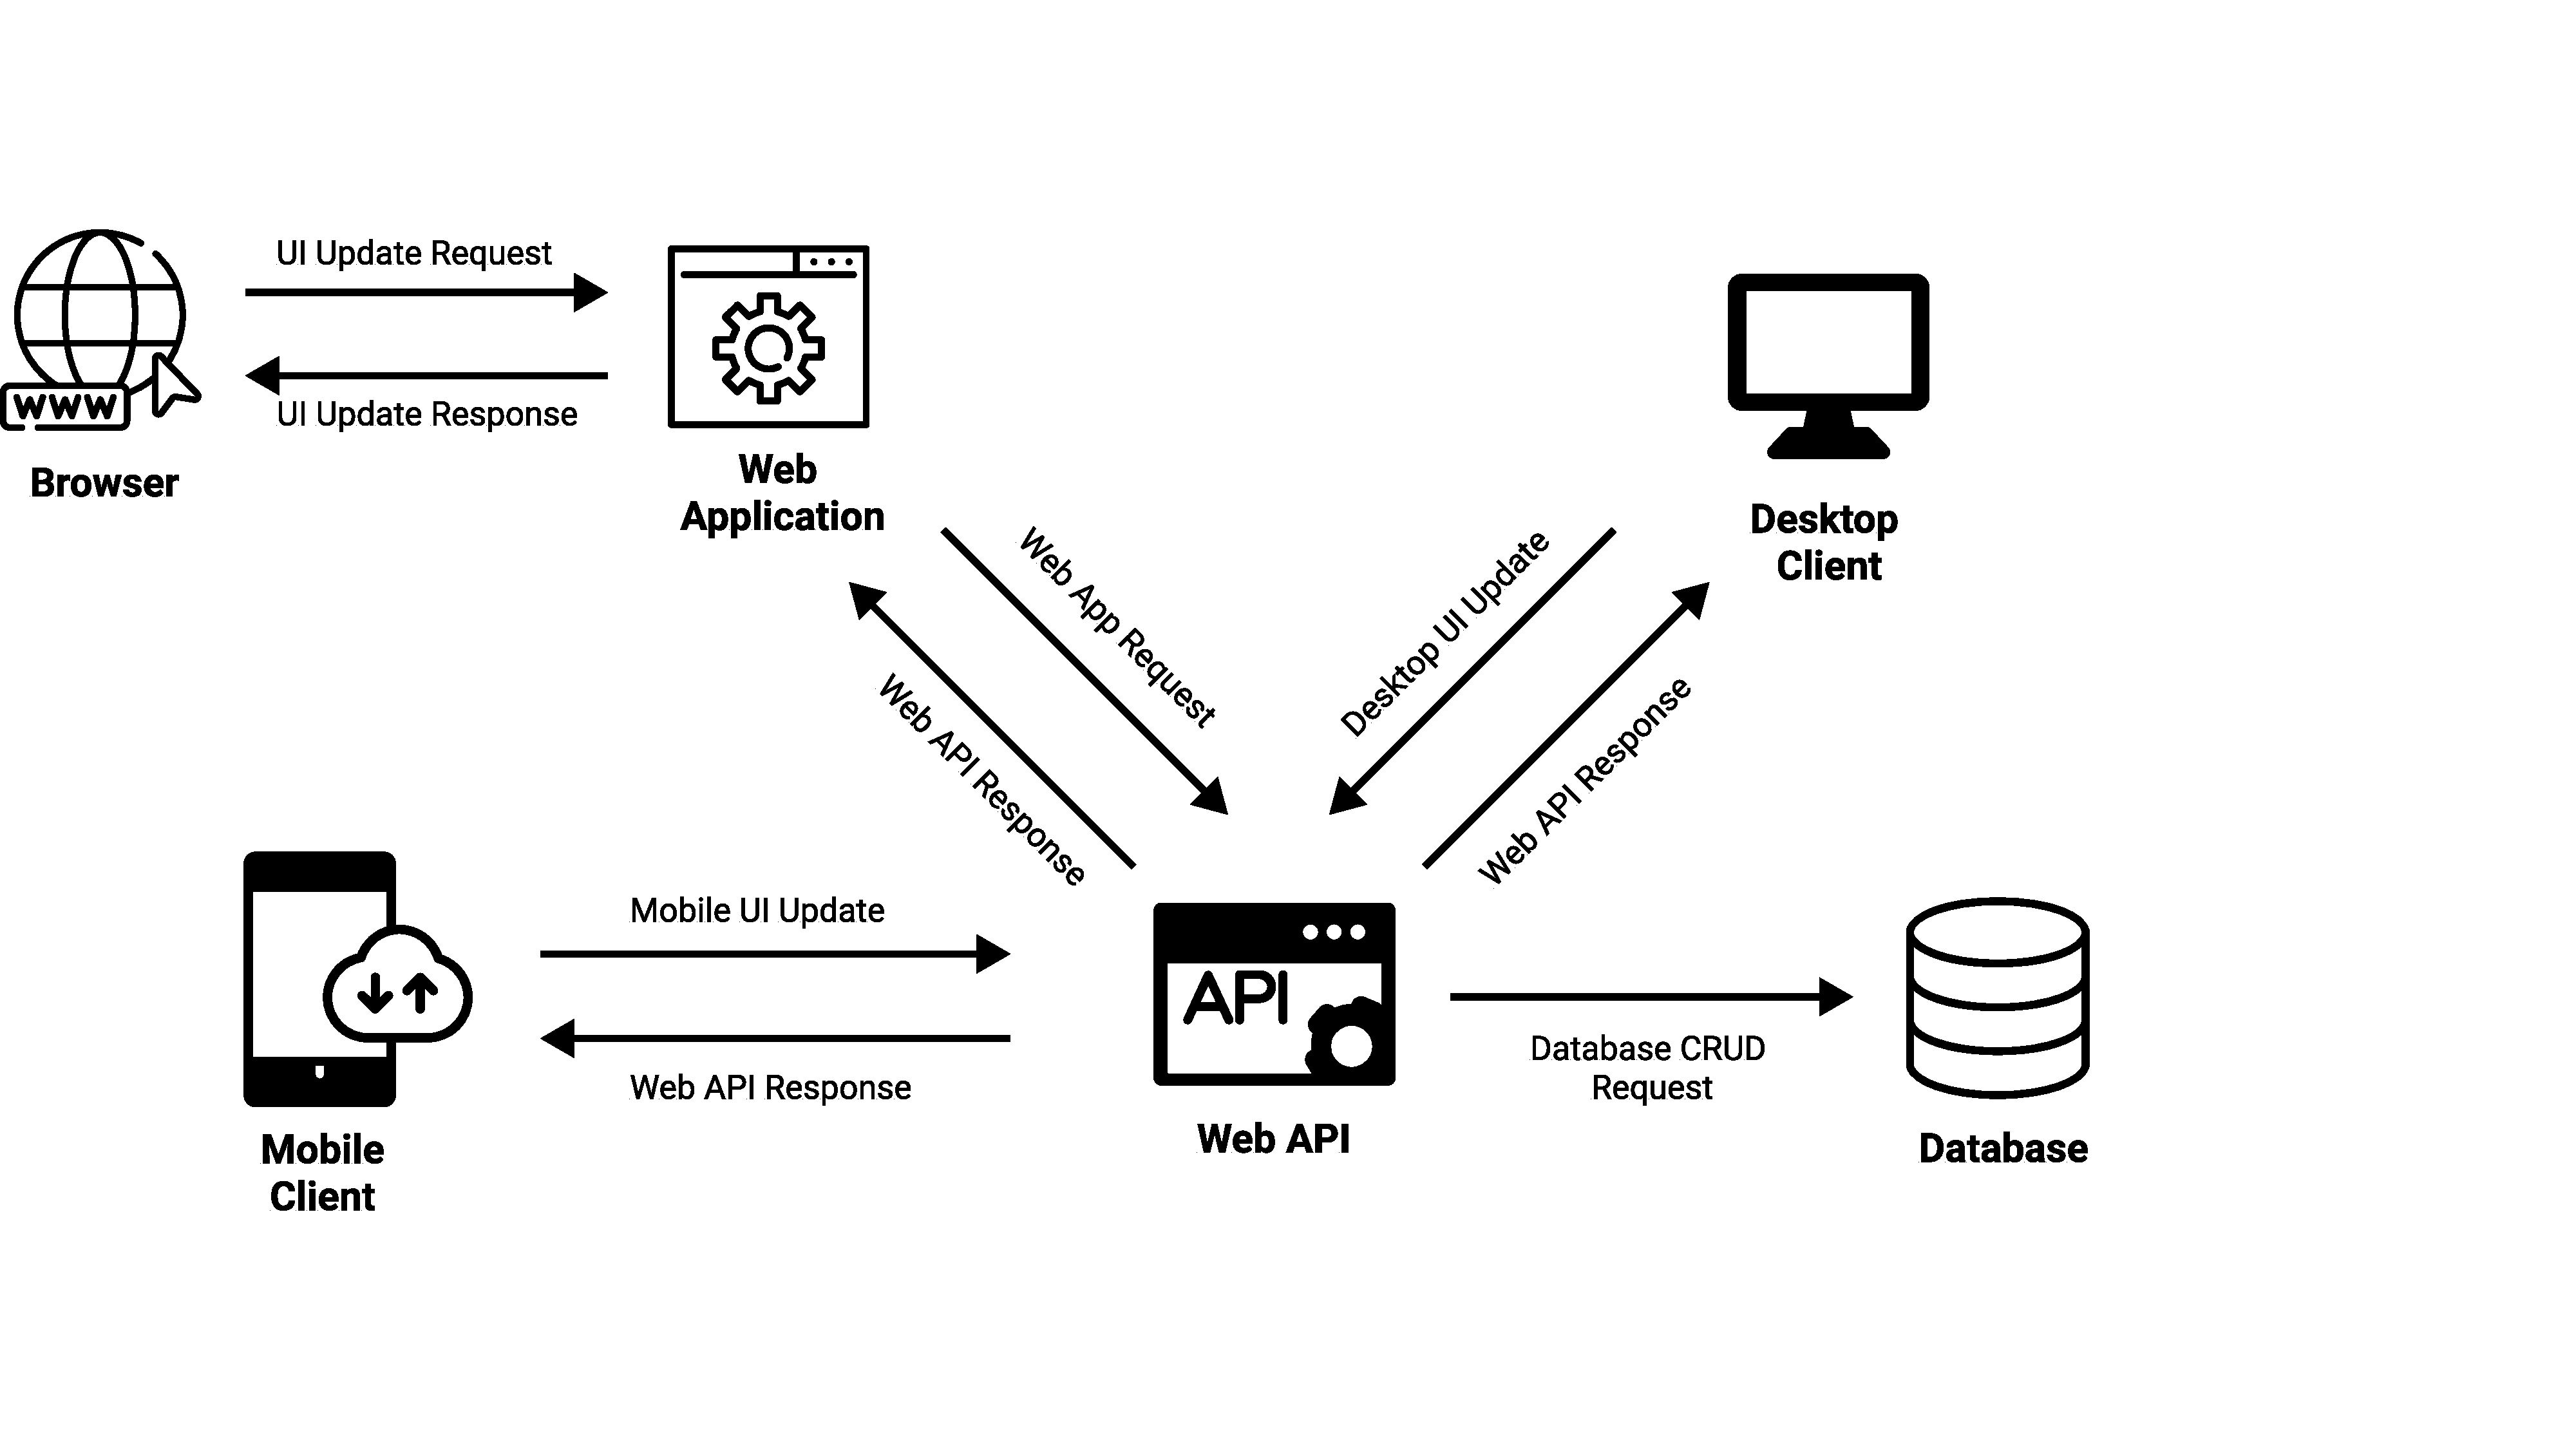
\includegraphics[width=1.2\textwidth]{Pictures/Threat_Modeling}
    \caption{Database diagram.}\label{fig:figure6}
\end{figure}

\begin{enumerate}
    \item \textbf{Browser UI Update Request}
    \begin{itemize}
        \item \textbf{Treat 1.1.} An adversary can perform action on behalf of other user due to lack of controls against cross domain requests.
        \item \textbf{Treat 1.2.} An adversary may bypass critical steps or perform actions on behalf of other users (victims) due to improper validation logic.
        \item \textbf{Treat 1.3.} An adversary can reverse weakly encrypted or hashed content.
        \item \textbf{Treat 1.4.} An adversary may gain access to sensitive data from log files.
        \item \textbf{Treat 1.5.} An adversary can spoof the target web application due to insecure TLS certificate configuration.
        \item \textbf{Treat 1.6.} An adversary can steal sensitive data like user credentials.
        \item \textbf{Treat 1.7.} An adversary can gain access to sensitive data stored in Web App's config files.
        \item \textbf{Treat 1.8.} An adversary can gain access to sensitive data by performing SQL injection through Web App.
        \item \textbf{Treat 1.9.} An attacker steals messages off the network and replays them in order to steal a user's session.
        \item \textbf{Treat 1.10.} An adversary can deface the target web application by injecting malicious code or uploading dangerous files.
        \item \textbf{Treat 1.11.} An adversary may spoof Desktop Web Browser (Chrome) and gain access to Web Application.
        \item \textbf{Treat 1.12.} An adversary can create a fake website and launch phishing attacks.
        \item \textbf{Treat 1.13.} Attackers can steal user session cookies due to insecure cookie attributes.
        \item \textbf{Treat 1.14.} An adversary can get access to a user's session due to insecure coding practices.
        \item \textbf{Treat 1.15.} An adversary can get access to a user's session due to improper logout and timeout.
        \item \textbf{Treat 1.16.} Attacker can deny the malicious act and remove the attack foot prints leading to repudiation issues.
        \item \textbf{Treat 1.17.} An adversary may gain access to sensitive data from uncleared browser cache.
        \item \textbf{Treat 1.18.} An adversary can gain access to sensitive information through error messages.
        \item \textbf{Treat 1.19.} An adversary can gain access to sensitive data by sniffing traffic to Web Application.
        \item \textbf{Treat 1.20.} An adversary can gain access to certain pages or the site as a whole.
        \item \textbf{Treat 1.21.} An adversary may gain access to unmasked sensitive data such as credit card numbers.
    \end{itemize}
    \item \textbf{Web App Request}
    \begin{itemize}
        \item \textbf{Treat 2.1.} An adversary may gain unauthorized access to Web API due to poor access control checks.
        \item \textbf{Treat 2.2.} An adversary can gain access to sensitive information from an API through error messages.
        \item \textbf{Treat 2.3.} An adversary can gain access to sensitive data by sniffing traffic to Web API\@.
        \item \textbf{Treat 2.4.} An adversary can gain access to sensitive data stored in Web API's config files.
        \item \textbf{Treat 2.5.} Attacker can deny a malicious act on an API leading to repudiation issues.
        \item \textbf{Treat 2.6.} An adversary may spoof Mango Web Application and gain access to Web API\@.
        \item \textbf{Treat 2.7.} An adversary may inject malicious inputs into an API and affect downstream processes.
        \item \textbf{Treat 2.8.} An adversary can gain access to sensitive data by performing SQL injection through Web API\@.
    \end{itemize}
    \item \textbf{Web API Response}
    \begin{itemize}
        \item \textbf{Treat 3.1.} An adversary can reverse weakly encrypted or hashed content.
        \item \textbf{Treat 3.2.} An adversary may gain access to sensitive data from log files.
        \item \textbf{Treat 3.3.} An adversary can gain access to sensitive information through error messages.
        \item \textbf{Treat 3.4.} Attacker can deny the malicious act and remove the attack foot prints leading to repudiation issues.
        \item \textbf{Treat 3.5.} An adversary can spoof the target web application due to insecure TLS certificate configuration.
        \item \textbf{Treat 3.6.} An adversary can steal sensitive data like user credentials.
        \item \textbf{Treat 3.7.} An adversary can create a fake website and launch phishing attacks.
    \end{itemize}
    \item \textbf{CRUD Request}
    \begin{itemize}
        \item \textbf{Treat 4.1.} An adversary can gain unauthorized access to database due to loose authorization rules.
        \item \textbf{Treat 4.2.} An adversary can gain access to sensitive PII or HBI data in database.
        \item \textbf{Treat 4.3.} An adversary can gain access to sensitive data by performing SQL injection.
        \item \textbf{Treat 4.4.} An adversary can deny actions on database due to lack of auditing.
        \item \textbf{Treat 4.5.} An adversary can tamper critical database securables and deny the action.
        \item \textbf{Treat 4.6.} An adversary may leverage the lack of monitoring systems and trigger anomalous traffic to database.
        \item \textbf{Treat 4.7.} An adversary can gain unauthorized access to database due to lack of network access protection.
    \end{itemize}
    \item \textbf{Mobile UI Update}
    \begin{itemize}
        \item \textbf{Treat 5.1.} An adversary can gain access to sensitive data by performing SQL injection through Web API.
        \item \textbf{Treat 5.2.} An adversary can reverse engineer and tamper binaries.
        \item \textbf{Treat 5.3.} An adversary may inject malicious inputs into an API and affect downstream processes.
        \item \textbf{Treat 5.4.} An adversary may spoof Mobile App (IOS, Android) and gain access to Web API\@.
        \item \textbf{Treat 5.5.} An adversary obtains refresh or access tokens from Mobile App (IOS, Android) and uses them to
        obtain access to the Mango Web API\@.
        \item \textbf{Treat 5.6.} Attacker can deny a malicious act on an API leading to repudiation issues.
        \item \textbf{Treat 5.7.} An adversary can gain access to sensitive data stored in Web API's config files.
        \item \textbf{Treat 5.8.} An adversary can gain sensitive data from mobile device.
        \item \textbf{Treat 5.9.} An adversary can gain access to sensitive data by sniffing traffic to Web API\@.
        \item \textbf{Treat 5.10.} An adversary can gain access to sensitive data by sniffing traffic from Mobile client.
        \item \textbf{Treat 5.11.} An adversary can gain access to sensitive information from an API through error messages.
        \item \textbf{Treat 5.12.} An adversary may gain unauthorized access to Web API due to poor access control checks.
        \item \textbf{Treat 5.13.} An adversary may jail break into a mobile device and gain elevated privilege.
    \end{itemize}
\end{enumerate}